% Aqu� se define el tama�o de letra principal:
\documentclass[12pt]{article}

% Configuro la codificación
\usepackage[utf8]{inputenc}		

%------------------------- Carga de paquetes ---------------------------
%
% Si no necesit�s alg�n paquete, comentalo.
%
% Definici�n del tama�o de p�gina y los m�rgenes:
%
\usepackage[a4paper,headheight=16pt,scale={0.7,0.8},hoffset=0.5cm]{geometry}


% Para escribir en castellano:
%
\usepackage[spanish]{babel}


%\usepackage{lstlang06}

%
% Si se prefiere tipograf�a Helvetica (Arial), descomentar las siguientes dos l�neas ( Las f�rmulas seguiran estando en Times)
%
%\usepackage{helvet}
%\renewcommand\familydefault{\sfdefault}
\usepackage{siunitx}
%
%------------------------- Carga de paquetes ---------------------------
%
% Si no necesit�s alg�n paquete, comentalo.
%
% Definici�n del tama�o de p�gina y los m�rgenes:
%
%\usepackage[a4paper,headheight=16pt,scale={0.7,0.8},hoffset=0.5cm]{geometry}

% Para escribir en castellano:
%
\usepackage[spanish]{babel}
%\usepackage[latin1]{inputenc}
%\usepackage{lstlang06}

%
% Si se prefiere tipograf�a Helvetica (Arial), descomentar las siguientes dos l�neas ( Las f�rmulas seguiran estando en Times)
%
%\usepackage{helvet}
%\renewcommand\familydefault{\sfdefault}
\usepackage{siunitx}
%
% El paquete amsmath agrega algunas funcionalidades extra a las f�rmulas. 
% Adem�s defino la numeraci�n de las tablas y figuras al estilo "Figura 2.3", en lugar de "Figura 7". (Por lo tanto, aunque no uses f�rmulas, si quer�s este tipo de numeraci�n dej� el paquete amsmath descomentado).
%
\usepackage{amsmath}
\usepackage{amsfonts} 
\usepackage{amssymb} 
\usepackage{fancybox} 
\numberwithin{equation}{section}
\numberwithin{figure}{section}
\numberwithin{table}{section}
\usepackage{listings}

%
% Para tener cabecera y pie de p�gina con un estilo personalizado:
%
\usepackage{fancyhdr}

%
% Para poner el texto "Figura X" en negrita:
% (Si no ten�s el paquete 'caption2', prob� con 'caption').
%
\usepackage[hang,bf]{caption}

%
% Para poder usar subfiguras: (al estilo Figura 2.3(b) )
%
\usepackage{subfigure}
%
% Para poder agregar notas al pie en tablas:
%
\usepackage{threeparttable}
\usepackage{multirow}

%------------------------------ graphicx ----------------------------------
%
% Para incluir im�genes, el siguiente c�digo carga el paquete graphicx 
% seg�n se est� generando un archivo dvi o un pdf (con pdflatex). 

% Para generar dvi, descoment� la linea siguiente:
%\usepackage[dvips]{graphicx}

% Para generar pdf, descoment� las dos lineas seguientes:
\usepackage[pdftex]{graphicx}
\pdfcompresslevel=9
\usepackage{float}
\usepackage{subfigure}
\usepackage{mathrsfs}
\usepackage{texdraw}
\usepackage{pdfpages}

%
%------------------------------ graphicx ----------------------------------

% Necesit�s este paquete si haces los diagramas de flujo en el programa Dia 
%\usepackage{tikz}
%\usepackage{standalone}
%\usepackage[all]{xy}

%\usepackage{pstricks,pst-node,pst-circ,pst-plot,pst-3dplot,pst-all}

% Hago que en la cabecera de p�gina se muestre a la derecha la secci�n,
% y en el pie, en n�mero de p�gina a la derecha:
%

%----------------------Encabezado y pie de página---------------------------%
\pagestyle{fancy}
%\renewcommand{\sectionmark}[1]{\markboth{}{\thesection\ \ #1}}

%Encabezado izquierdo
\lhead{\miAsignatura}
%Encabezado derecho
\rhead{
\includegraphics[scale=0.2]{./Logos/Logo_FIUBA_2}}
%Pie de p�gina izquierdo
\lfoot{\miCuatri}
%Pie de p�gina central
\cfoot{}
%Pie de p�gina derecho
\rfoot{Página:\thepage}
%L�nea de la nota de pie
\renewcommand{\footrulewidth}{0.4pt}
% En el siguiente archivo se configuran las variables del trabajo práctico
%% \providecommand es similar a \newcommnad, salvo que el primero ante un 
%% conflicto en la compilación, es ignorado.

% Al comienzo de un TP se debe modificar los argumentos de los comandos

\providecommand{\miTitulo}{Tp de simulación I}
\providecommand{\miSubtitulo}{Repetidor Analógico vs Repetidor Digital}

\providecommand{\miAsignatura}{Procesos Estocásticos (86.09)}

\providecommand{\miAlumnoUno}{Alcaraz, Gonzalo}
\providecommand{\miMailAlumnoUno}{g.alcaraz@outlook.com}
\providecommand{\miPadronUno}{93874}

\providecommand{\miAlumnoDos}{Chaparro, Raúl Antonii}
\providecommand{\miMailAlumnoDos}{chaparroraulantonio@gmail.com	}
\providecommand{\miPadronDos}{96222}

\providecommand{\miAlumnoTres}{Alcaraz, Gonzalo}
\providecommand{\miMailAlumnoTres}{g.alcaraz@outlook.com}
\providecommand{\miPadronTres}{93874}

\providecommand{\miAlumnoCuatro}{Apellido, Nombre}
\providecommand{\miMailAlumnoCuatro}{Mail}
\providecommand{\miPadronCuatro}{Padron}

\providecommand{\miNumGrupo}{3}

% No es necesario modificar este
%\providecommand{\myHeaderLogo}{header_fiuba}

\providecommand{\miAutores}{Alcaraz & Chaparro}
\providecommand{\miCuatri}{Año 2017 - 2\textsuperscript{do} Cuatrimestre}
\providecommand{\miFecha}{18 de Octubre del 2017}
% Título y autor(es):

\title{Trabajo práctico 1}
\author{Alcaraz, Chaparro}

%------------------------- Comandos útiles --------------------------------


%------------------------- Inicio del documento ---------------------------

\begin{document}

	% Carátula:
%
\begin{titlepage}
	
	\thispagestyle{empty}
	
	\begin{center}
		
\includegraphics[scale=1]{./Logos/Logo_FIUBA_1}\\
		\large{\textsc{Universidad de Buenos Aires}}\\
		\large{\textsc{Facultad De Ingenierí­a}}\\
		\small{\miCuatri}
	\end{center}
	
	\vfill
	
	\begin{center}
		\Large{\underline{\textsc{\miAsignatura}}}
	\end{center}
	
	\vfill
	
	\begin{tabbing}
		\hspace{2cm}\=\+\miTitulo\\
		TEMA: \miSubtitulo.\\
		FECHA: \miFecha\\
		\\
		INTEGRANTES:\hspace{-1cm}\=\+\hspace{1cm}\=\hspace{6cm}\=\\
		\miAlumnoUno \>\>- \miPadronUno\\
		\>\footnotesize{$<$\miMailAlumnoUno$>$}\\
		\miAlumnoDos	\>\>- \miPadronDos\\
		\>\footnotesize{$<$\miMailAlumnoDos$>$}\\
				
		%APELLIDO3, Nombre3	\>\>- \#88888\\
		%	\>\footnotesize{$<$nombre3\_apellido3@dominio.com$>$}\\
		
	\end{tabbing}
	
	\hspace{1cm} GRUPO: \miNumGrupo
	%\vfill
	
	%\hrule
	%\vspace{0.2cm}
	
	%\noindent\small{66.08 - Circuitos I \hfill}
	
\end{titlepage}
	
	% Hago que las p�ginas se comiencen a contar a partir de aca:
	\pagestyle{fancy}
	
	\setcounter{page}{1}
	
	
	% Pongo el �dice en una p�gina aparte:
	\newpage
	
	\tableofcontents
	
	% Inicio del TP:
	\newpage
	\section{Introducción}
		
			\indent En el siguiente trabajo práctico se analizará dos esquemas de comunicaciones, uno digital y otro analógico. En ambos casos se transmitirán símbolos que representan 1 bit. Si el bit es 1, el símbolo será A y si es 0 se simbolorizá -A. La probabilidad de que A se 1 o 0 es $\frac{1}{2}$. En cada etapa de estos sistemas de comunicación a la señal se la mutltiplica por un atenuador \emph{h} y se le suma un ruido $W \sim N(0,\sigma ^2)$\\
	
	\indent En el \textbf{repetidor digital}, que se ilustra en la figura \ref{Fig.Sist_dig}, el bloque con la letra \textbf{D} toma una decisión acerca del símbolo transmitido y lo retransmite a la etapa siguiente y es la última etapa donde el detector toma la desición final. La opereación matemática del detector \textbf{D} se puede escribir como:
	
						\begin{equation}
							X_{i+1}=
									\begin{cases}
											A		& \quad \text{si} Y_i \geq 0 \\
											-A		& \quad \text{si} Y_i \leq 0
									\end{cases}
						\label{Eq.sis.digital}
						\end{equation}

	\indent En cambio en el \textbf{repetidor analógico}, cuya representación es la de la Figura \ref{Fig.Sist_ana}, se toma una única decisión y ocurre en el receptor. En los casos intermedios, los símbolos recibidos son multiplicados por una ganancia para luego retransmitirlos a la siguiente estapa. Dichos símbolos se pueden representar según:
	
						\begin{equation}
							x_{I+1} = G_{i+1} \cdot Y_i \quad i=1,....,n-1
							\label{Eq.sis.analogico}
						\end{equation}
						
			\begin{figure}[H]
				\centering
				\begin{subfigure}[b]{0.7\textwidth}
					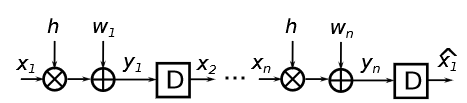
\includegraphics[width=\textwidth]{./Figuras/Sistema_digital}
					\caption{Sistema de comunicación digital}
					\label{Fig.Sist_dig}
				\end{subfigure}
			\begin{subfigure}[b]{0.7\textwidth}
				\includegraphics[width=\textwidth]{./Figuras/Sistema_analogico}
				\caption{Sistema de comunicación analógico}
				\label{Fig.Sist_ana}
			\end{subfigure}
			\caption{Sistemas de comunicaciones con distintos tipos de repetidores}
		\end{figure}
	
	\section{Desarrollo}	
		\subsection{Ejercicio 1: Cálculo de ganancia de los repetidores analógicos}
	
			\indent Se asume que cada repetidor analógico puede transmitir como máximo con una energía $\varepsilon$ .Por lo tanto se puede decir: $\sigma _{X_i}^{2} = \mathbb{V}[X_i] = A^2$. \\
\indent Tomando por ejemplo el caso i =1, según la ecuación \ref{Eq.sis.analogico}, para $X_2 = G_2 \cdot Y_1  \Rightarrow \mathbb{V}[X_2] = \varepsilon = \mathbb{V}[G_2 \cdot Y_1] = \mathbb{V}[G_2 \cdot (h \cdot X_1 + W_1)]$. Como puedo suponer que X es independiente al ruido W, puedo aplicar la propiedad de la varianza, $\mathbb{V}[\alpha X]= \alpha^2 \cdot \mathbb{V}[X]$ y la propiedad de la suma $\mathbb{v}[X+Y] = \mathbb{V}[X]+ \mathbb{V}[Y]$. Al aplicar dichas propiedades la expresión me queda:

				\begin{equation}
					\mathbb{V}[X_2] =(G_2 \cdot h)^2 \cdot \mathbb{V} [X_1] + G_2^2 \cdot \mathbb{V}[ W_1]
				\label{Eq.VarX2}
				\end{equation}  
	
\indent Trabajando algebráicamente la ecuación \ref{Eq.VarX2}, me queda $\mathbb{V}[X_2] = G_2^2 \cdot (h^2 \cdot \mathbb{V}[X_1] + \mathbb{V}[W_1])$. Como la $\mathbb{V}[X_1] = \varepsilon$ y $W \sim N(0,\sigma ^2)$, la expresión anterior se puede expresar como $G_2^2 = \frac{\varepsilon}{h^2 \cdot \varepsilon \sigma ^2}$. Como las $X_i$ tendrán la misma energía y las $W_i$ se distribuyen normalmente identicamente e independientes, se puede generalizar de tal forma que queda:
				\begin{equation}
					G_i = \sqrt{\frac{\varepsilon}{h^2 \cdot \varepsilon + \sigma ^2}}
				\label{Eq.Gi}
				\end{equation}

Se pide expresar la ecuación anterior en función de la relación señal a ruido, $SNR = h^2 \cdot \varepsilon / \sigma ^2$. Sacando $\sigma$ de factor común y multiplicando y dividiendo por $h^2$, me queda:
			
				\begin{align}
					G_i &= \sqrt{\frac{\textcolor{red}{h^2} \cdot \varepsilon}{\sigma ^2 \cdot \textcolor{red}{h^2} \cdot (\frac{h^2 \cdot \varepsilon}{\sigma ^2} + 1)}} \\
					G_i &= \sqrt{\frac{SNR}{h^2 \cdot (SNR + 1)}}
					\label{Eq.Gi_SNR}
				\end{align}
Como $\mathbb{V}[X_1] = A^2$, la ecuacion \ref{Eq.Gi} la podemos expresar como: $G_2 ^2 = \frac{\varepsilon}{h^2 \cdot A^2 + \sigma ^2} \Rightarrow A = \sqrt{(\frac{\varepsilon}{G_2^2}-\sigma ^2)/h^2}$. Trabajando la expresión anterior:

				\begin{align}
					A &= \sqrt{\frac{h^2 \cdot \varepsilon}{G_2^2}- h^2 \cdot \sigma ^2} \\	
					A &= \sqrt{\sigma ^2 \cdot (\frac{h^2 \cdot \varepsilon}{G_2^2 \cdot \sigma ^2}- h^2)} \\
					A &= \sigma \cdot \sqrt{\frac{SNR}{G_2^2}-h^2}
					\label{Eq.A_SNR}
				\end{align}
			
\indent De esta forma en las ecuaciones \ref{Eq.Gi_SNR} y \ref{Eq.A_SNR} expresamos el valor de A y de las ganancias en función de la relación señal ruido.

		
		\subsection{Ejercicio 2: Probabiliad de error del sistema analógico}
		
			\indent Como se puede ver en la figura ref{Agregar figura en la introduccion} $Y_n = h \cdot X_n + W_n $, y según la ecuación \ref{Eq.sis.analogico}  $ X_n = G_n \cdot Y_{n-1} \Rightarrow Y_n = h \cdot (G_n \cdot Y_{n-1})+ W_n$. Luego,  $Y_n = h \cdot (G_n \cdot (h \cdot X_{n-1} + W_{n-1})) + W_n $. Al mismo tiempo según la expresión \ref{Eq.sis.analogico} $X_{n-1} = G_{n-1} \cdot Y_{n-2} = G_{n-1} \cdot (h \cdot X_{n-2} + W_{n-2})$. Subsituyendo esta última expresión en la ecuación de $Y_n$ se obtiene:

		\begin{equation}
			y_n = h^3 \cdot G_n \cdot G_{n-1} \cdot X_{n-2} + h^2 \cdot G_n \cdot G_{n-1} \cdot W_{n-2} + h \cdot G_n \cdot G_n \cdot W_{n-1} + W_n
			\label{Eq.yn}			
		\end{equation}

\indent Por recurrencia, se puede obtener la sigueinte expresión compacta de $Y_n$

		\begin{equation}
				Y_n = \left(\prod_{i=2}^{n}{h \cdot G_i} \right) \cdot X_i + \left( \sum_{j=1}^{n-1} \left( \prod_{k=j+1}^{n} h \cdot G_k \right) \cdot W_j \right) + W_n
				\label{Eq.YN}
		\end{equation}
		
\indent En la ecuación \ref{Eq.YN} se notan dos partes bien definidas y de las cuales $Y_n$ depende. Estas son, el primer término $X_1$ y el segundo término del ruido $W_n$. Se sabe por condiciones de enunciado que el ruido tiene una distribución normal. Como se ve en la expresión \ref{Eq.YN} el segundo termino es una sumatoria de $W_n$, por lo tanto ese término tiene una distrbucion normal de media nula y varianza: $\left( h \cdot G \right)^{2 \cdot (n-1)} \cdot \sigma ^2$, es decir $\left( \sum_{j=1}^{n-1} \left( \prod_{k=j+1}^{n} h \cdot G_k \right) \cdot W_j \right) + W_n \sim N (0, \left( h \cdot G \right)^{2 \cdot (n-1)} \cdot \sigma ^2)$.\\

\indent Por comodidas, como las ganancias G y las atenuaciones h son las mismas en todas las etapas, podemos escribir la ecuacion \ref{Eq.YN} de la sigueinte manera:

			\begin{equation}
				Y_n = h^n \cdot G^{n-1} \cdot X_1 + \sum_{j=1}^{n} \left( h \cdot G \right)^{n-j} \cdot W_j
				\label{Eq.Yreducida}
			\end{equation}

\indent Para calcular la relacipon señal a ruido de la última etapa se puede partir de la ecuación \ref{Eq.q.YN} y como X y W son independientes se puede escrbir:

			\begin{align*}
				\mathbb{V}[Y_n] &= \mathbb{V}\left[ \left(\prod_{i=2}^{n}{h \cdot G_i} \right) \cdot X_i + \left( \sum_{j=1}^{n-1} \left( \prod_{k=j+1}^{n} h \cdot G_k \right) \cdot W_j \right) + W_n \right] \\
				\mathbb{V}[Y_n] &= h^{2n} \cdot G^{2(n-1)} \cdot \mathbb{V}[X_1] + \sum_{j=1}^{n} \left( (h \cdot G)^{2(n-j)} \cdot \mathbb{V}[W_j] \right)
			\end{align*}
\indent Asumiendo que $\mathbb{V}[X_1] = \sigma _{X_1}^2 = \varepsilon$ y que $\mathbb{V}[X_j] = \sigma ^2$ la ecuación anterior la podemos excribir como

			\begin{equation}
				mathbb{V}[Y_n] = h^{2n} \cdot G^{2(n-1)} \cdot \varepsilon + \sum_{j=1}^{n} \left( (h \ cdot G)^{2(n-j)} \cdot \sigma ^2 \right)
				\label{Eq.VarYn}
			\end{equation}
			
\indent Si se observa en la ecuación \ref{Eq.VarYn} la varianza de la señal de interés es la suma de la varianza de la señal de entrada y la suma de los ruidos (salvo constantes). Como la relación de la señal a ruido se define comoel cociente entre la energía  de la señal de interés y la varianza del ruido, en este caso queda:
	
			\begin{align*}
			\textbf{SNR}(n) &=\frac{h^{2n} \cdot G^{2(n-1) } \cdot \varepsilon}{\sum_{j=1}^{n} \left[h \cdot G \right] ^{2(n-j)} \cdot \sigma ^2} \\
			\textbf{SNR}(n) &= \frac{\left(h \cdot G \right) ^{2n} \cdot G^{-2} \cdot \varepsilon}{\left(h \cdot G \right) ^{2n} \cdot \sigma ^2 \cdot \sum_{j=1}^{n} \left[ (h \cdot G) ^{-2} \right] ^j }
			\end{align*}
			
\indent Aplicando la identidad: $\sum_{^j=a}^{b}q^j = \frac{q^a - 1^{b+1}}{1 - q}$, la ecuación anterior se puede expresar como:

			\begin{align*}
				\textbf{SNR}(n) &= \frac{G^{-2} \cdot \varepsilon}{\sigma ^2 \cdot \frac{(h \cdot G)^{-2} -(h \cdot G)^{-2(n+1)}}{1-(h \cdot G)^{-2}}} \\
				\textbf{SNR}(n) &= \frac{\varepsilon \cdot (1-(h \cdot G)^{-2})}{\sigma ^2 \cdot h^{-2} (1 - (h \cdot G)^{-2n})}\\
			\end{align*}

\indent Como $G^2 = \frac{\varepsilon}{h^2 \cdot \varepsilon + \sigma ^2}$, la relación de la señal a ruido de la última etapa se puede reescribir como:

			\begin{align*}
				\textbf{SNR}(n) &= \frac{\varepsilon \cdot (1- h^{-2} \cdot \left( (h^2 \cdot \varepsilon + \sigma ^2 ) / \varepsilon \right) }{h^{-2} \cdot \sigma ^2 \cdot \left[ 1- h^{-2n} \cdot \left( \frac{h^2 \cdot \varepsilon + \sigma ^2}{\varepsilon} \right) ^n \right]} \\
				\textbf{SNR}(n) &= \frac{- \sigma ^2 \cdot h^{-2}}{\frac{h^{-2} \cdot \sigma ^2}{\varepsilon ^n} \cdot [\varepsilon ^n - h^{-2n} \cdot (h^2 \cdot \varepsilon + \sigma ^2)^n]} \\
				\textbf{SNR}(n) &= \frac{- \varepsilon ^n}{\varepsilon ^n - \left( \frac{h^2 \cdot \varepsilon + \sigma ^2}{h^2} \right) ^n}			
			\end{align*}
	
\indent Se pide calcular la probabilidad de error ($p_e$), que sería $p_e = P(X \neq \widehat{X})$. Usando probabilidad total y que X puede ser A o -A se obtiene:

			\begin{equation}
				P_e = \mathbb{P}(X_1 \neq \widehat{X_1} | X_1 = A) \cdot \mathbb{P}(X_1 =A) + \mathbb{P} (X_1 \neq \widehat{X_1} | X_1 = -A) \cdot \mathbb{P}(X_1 = -A)
				\label{Eq.prob_e}
			\end{equation}

\indent	Como dato se tiene que $\mathbb{P}(X_1 = A) = \mathbb{P}(X_1 = -A) = 0.5$ y reescribiendo la ecuación \ref{Eq.prob_e}:

			\begin{align}
				P_e &= \mathbb{P}(X_1 \neq A | X_1 = A) \cdot \frac{1}{2} + \mathbb{P} (X_1 \neq -A | X_1 = -A) \cdot \frac{1}{2} \\
				P_e &= \mathbb{P}(Y_n \leq 0 | X_1 = X_{n+1}) \cdot \frac{1}{2} + \mathbb{P} (y_n > 0 | X_1 = X_{n+1}) \cdot \frac{1}{2} 
				\label{Eq.proba_e2}
			\end{align}

\indent Tomando el primer término multiplicado por 2 de la ecuación \ref{Eq.proba_e2} y subtituyendo según la ecuación \ref{Eq.Yreducida}
			
			\begin{align*}
				\mathbb{P}(X_1 \neq A | X_1 = A) &= \mathbb{P}\left( h^n \cdot G^{n-1} \cdot X_1 + \sum_{j=1}^{n}(h \cdot G)^{n-j} \cdot W_j |X_1=A \right)	\\
				\mathbb{P}(X_1 \neq A | X_1 = A) &= \mathbb{P} \left( \sum_{j=1}^{n} (h \cdot G)^{n-j} \cdot W_j \leq -A h^n \cdot G^{n-1} \right)		
			\end{align*}
\indent Realiznado el siguiente cambio de varible: $\beta = \sum_{j=1}^{n} (h \cdot G)^{n-j} \cdot W_j$ donde $\beta$	al ser una suma de normales sigue teniendo una distribución normal. Por lo tanto si llamo $Z= \frac{\beta - \mathbb{E}[\beta]}{\sqrt{\mathbb{V}[\beta]}}$, $Z \sim N(0,1)$. Por lo tanto lo buscado, en esta parte es:

			\begin{equation}
				\mathbb{P}(X_1 \neq A | X_1 = A) = \mathbb{P} \left( Z\leq - \left(\frac{A \cdot h^n \cdot G^{n-1} + \mathbb{E}[\beta]}{\mathbb{V}[\beta]} \right) \right)
				\label{Eq.Prob.Beta} \\
			\end{equation}

\indent Ahora bien, $\beta = \sum_{j=1}^{n-1} (h ^\cdot G)^{n-1} \cdot W_j = \begin{bmatrix} (h \cdot G)^{n-1}, .... 1 \end{bmatrix} \cdot \begin{bmatrix} W_1, W_2, ...., W_j \end{bmatrix} ^T = \underline{D^T} \cdot \underline{W}$. Como $\underline{W} \sim N(0,C_W) \Rightarrow \beta \sim N(0, G \cdot C_W \cdot G^T)$. Por lo tanto

				\begin{align*}
				\mathbb{V}[\beta] &= \begin{bmatrix} (h \cdot G)^{n-1}, \cdots ,1 \end{bmatrix} \begin{bmatrix} \sigma ^2 & 0 & \cdots & 0 \\ 0 & \sigma ^2 & \cdots & 0 \\ \vdots & \vdots & \ddots & \vdots \\ 0 & 0 & \cdots & \sigma ^2\end{bmatrix} \cdot \begin{bmatrix} (h \cdot G)^{n-1}\\ \vdots \\ 1 \end{bmatrix} \\
				\mathbb{V}[\beta] &= \sigma ^2 \cdot \sum_{j=1}^{n}(h \cdot G)^{2(n-j)}
				\end{align*}

\indent Por simetría el segundo término de la ecuación \ref{Eq.proba_e2} es similar a la expresión \ref{Eq.Prob.Beta}, y como ambos términos de la ecuación \ref{Eq.proba_e2} están multiplicados por $\frac{1}{2}$, termina dando

				\begin{equation}
				\mathbb{P}(X_1 \neq \widehat{X_1}) = 1 - \phi \left( \frac{A \cdot h^n \cdot G^{n-1}}{\sqrt{\sigma ^2 \cdot \sum_{j=1}^{n} (h \cdot G)^{2(n-j)}}}	 \right) 
				\end{equation}		

\indent En el ejercicio se pide calcular dicha propiedad pero en términos de \textbf{SNR}. Con la expresión recién encontrada, teniendo en cuenta los resultados del punto 1 (ecuaciones \ref{Eq.Gi_SNR} y \ref{Eq.A_SNR}) y trabajando algebraicamente se puede obtener:

				\begin{equation}
<<<<<<< HEAD
					\mathbb{P}(X_1 \neq \widehat{X_1}) = 1 - \phi \left( \frac{h^2 \cdot \sqrt{\textbf{SNR}^n}}{\sqrt{(\textbf{SNR}+1)^n -\textbf{SNR}^n}} \right)= Q \left( \frac{h^2 \cdot \sqrt{\textbf{SNR}^n}}{\sqrt{(\textbf{SNR}+1)^n -\textbf{SNR}^n}} \right)
=======
					\mathbb{P}(X_1 \neq \widehat{X_1}) = 1 - \phi \left( \frac{h^2 \cdot \sqrt{\textbf{SNR}^n}}{\sqrt{(\textbf{SNR}+1)^n -\textbf{SNR}^n}} \right)
>>>>>>> origin/master
					\label{Eq.prob_SNR}					
				\end{equation} 	
		
		\subsection{Ejercicio 3: Probabilidad de error del sistema digital}
		
			En la figura \ref{fig:prob_err} se muestra la probabilidad de error de ambos sistemas en función de la \textit{SNR}, en casos de distintas cantidades de repetidores. Las curvas del sistema analógico se hicieron en base a un $h=1$ (figura \ref{fig:prob_err_a}) y $h=0.5$ (figura \ref{fig:prob_err_b}) para ilustrar la influencia del mismo sobre la probabilidad del error. El error en el sistema digital no depende del valor de $h$.


\begin{figure}[]
    \centering
    \begin{subfigure}[t]{0.8\textwidth}
        \centering
        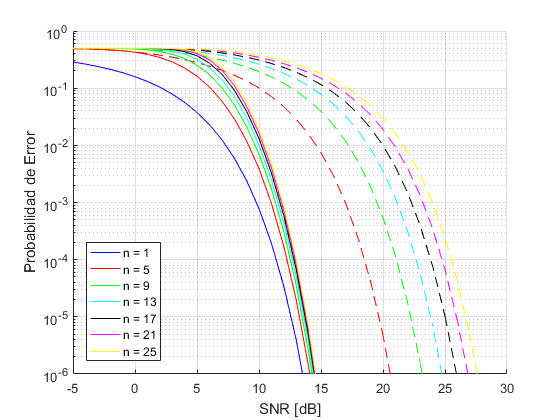
\includegraphics[width=\textwidth]{./Matlab/ej3h=1.png}
        \caption{$h=1$}
        \label{fig:prob_err_a}
    \end{subfigure}%
    \\
    \begin{subfigure}[t]{0.8\textwidth}
        \centering
        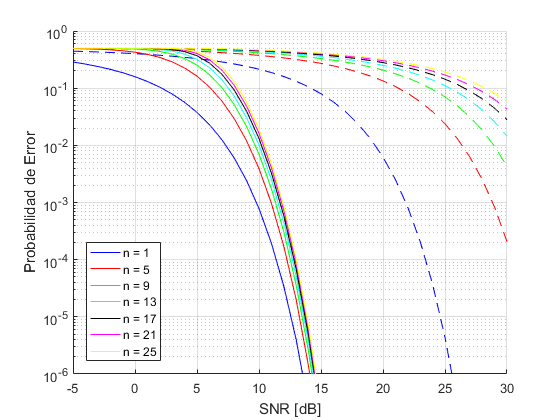
\includegraphics[width=\textwidth]{./Matlab/ej3h=05.png}
        \caption{$h=0.5$}
        \label{fig:prob_err_b}
    \end{subfigure}
    \caption{Probabilidad de error en función del SNR. La línea punteada representa el sistema analógico, y la continua el digital.}
\label{fig:prob_err}
\end{figure}

Para ambos sistemas, independientemente del valor de $h$ y para cada $n$, ocurren cuando $\textbf{SNR}=\SI{-5}{\decibel}$. Mientras menor es el valor de \textbf{SNR} y $n$, más parecido es el error en ambos sistemas (siendo idéntico en el caso en que $n=1$), lo cual resulta claro a partir de las expresiones matemáticas. A su vez, a medida que se tiene un valor menor de $h$, mayor es el error del sistema analógico. 

Teniendo esto en cuenta, resulta evidente elegir el sistema digital, debido a su menor probabilidad de error.

También se observa que al agregar repetidores (valor mayor de $n$), las curvas se abren más, reflejando el agregado de fuentes de ruido. Este hecho resulta más evidente en el caso del sistema analógico. Esto podría deberse en parte al fenómeno de que el error de una etapa digital compense el error de otra. 

La fórmula de probabilidad de error para el sistema digital puede demostrarse a partir de un argumento por recurrencia. Se parte de la fórmula de probabilidad de error para un sistema de un solo repetidor, la cual toma la siguiente forma:

\begin{equation}
P_{e,1}=\mathbb{P}(X_2\neq X_1) 
\end{equation} 

Esta probabilidad es igual a $Q(\sqrt{\textbf{SNR}})$. Si se agrega otro repetidor, se tiene que

\begin{equation}
P_{e,2}=\mathbb{P}(X_3\neq X_1)=\mathbb{P}(X_3\neq X_2)\mathbb{P}(X_2 = X_1)+\mathbb{P}(X_3 = X_2)\mathbb{P}(X_2\neq X_1)
\end{equation} 

lo que equivale a 

\begin{equation}
P_{e,2}=P_{e,1}(1-P_{e,1})+(1-P_{e,1})P_{e,1}
\end{equation} 

dado que $X_2 = X_1$ es complementario al error, y $X_3 \neq X_2$ es probabilidad de error con un solo repetidor. Con esto puede generalizarse que para $n$ repetidores vale

\begin{equation}
P_{e,n}=P_{e,1}+P_{e,n-1}-2P_{e,1}P_{e,n-1}
\end{equation} 

Ahora bien, esto es una ecuación en diferencias con condición inical $P_1 = Q(sqrt{SNR})$. 

Para continuar operando y por comodidad, se llamarán $x[n]=P_{e,1},\alpha=P_{e,1},\beta=1-2P_{e,1}$. Se reescribe la ecuación anterior de la siguiente forma:

\begin{equation}
x[n]-\beta x[n-1]=\alpha
\end{equation} 

con solución de la ecuación homogénea $x_H[n]=k\beta^n$, con $k \in \mathbb{R}$ dependiendo de la condición inicial. Se propone $x_P[n]=c$ como solución particular, con $c\in\mathbb{R}$. Reemplazando, se obtiene que 

\begin{equation}
c=\frac{\alpha}{1-\beta}
\end{equation} 

Sumando ambas soluciones para obtener la solución a la ecuación, y con la condición inicial, se obtiene que 

\begin{equation}
k = \frac{P_{e,1}}{\beta}-\frac{\alpha}{\beta-\beta^2}
\end{equation} 

Siendo entonces la solución

\begin{equation}
x[n]=(\frac{P_{e,1}}{\beta}-\frac{\alpha}{\beta-\beta^2})\beta^n+\frac{\alpha}{1+\beta}
\end{equation} 

Finalmente, reemplazando los valores de $\alpha,\beta,P_{e,1}$ se llega a la expresión de probabilidad de error para un sistema digital

\begin{equation}
P_{e,n}=\frac{1}{2}(1-(1-2Q(\sqrt{\textbf{SNR}})^n))
\end{equation} 
		
		\subsection{Ejercicio 4: Simulacion Monte Carlo de las probabilidades de error}
			
			La figura \ref{fig:mc_h1} muestra la probabilidad de error para ambos sistemas en base a una simulación Montecarlo, y las curvas teóricas para comparar. Se tomo un valor de $h=1$.

\begin{figure}[]
    \centering
    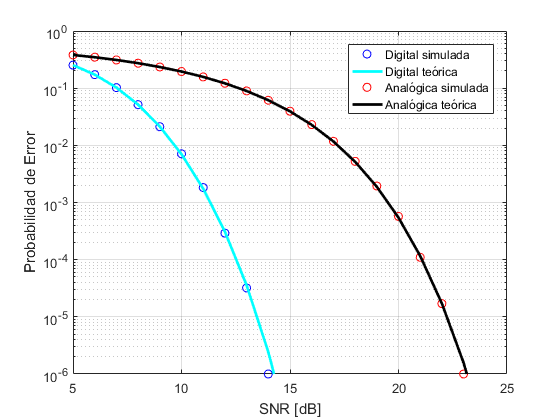
\includegraphics[width=\textwidth]{./Matlab/ej4h=1n=1meg.png}
    \caption{Probabilidad de error en función del SNR, simulada y teórica. }
\label{fig:prob_err}
\end{figure}

Puede verse que las curvas teóricas corresponden con muy buena precisión a los puntos simulados. Esto se debe a que, al generarse una cantidad muy grande de entradas simuladas, el cociente de errores y realizaciones aproxima estadísticamente la probabilidad del error.

En particular, este gráfico se generó con un millón de realizaciones para cada sistema y valor de \textbf{SNR}; sin embargo, se observó que a partir de aproximadamente veinte mil realizaciones puede notarse una clara tendencia a aproximarse a las curvas teóricas. 
			
		\section{Conclusiones}			
La aplicación de herramientas matemáticas de análisis permitieron hacer varias observaciones acerca de la confiabilidad de los sistemas digitales y analógicos para transmitir información. 

En primer lugar, resulta incuestionable que los sistemas digitales presentan menor probabilidad de error de transmisión que los analógicos. Este resultado podría haberse intuido \textit{a priori}, ya que en el sistema digital cada etapa toma una decisión, la cual depende mayormente del ruido que haya sido introducido en la misma; por otro lado, el sistema analógico amplifica el ruido en cada etapa, aumentando considerablemente el error. El análisis probabilístico plasmado en los gráficos permite confirmar este fenómeno con mayor rigurosidad.

Pudo comprobarse además que el método de simulación Monte Carlo converge a la curva teórica a medida que aumenta la cantidad de muestras simuladas, con lo que se pudo verificar la utilidad del mismo.
\end{document}
